\section{The IIM for the advection equation}
In this section, we will explore the IIM for solving the advection equation in one dimension with a non-smooth initial condition

\subsection{The IIM for a wedge initial condition}

We will solve the advection equation

\begin{equation}
    \frac{\partial u}{\partial t} = -a \frac{\partial u}{\partial x}
\end{equation}

on $0 \leq x \leq 1$ using a number of methods.

The parameters of this problem are:

interface at $x = \alpha(t)$ where

\begin{equation}
    \alpha(t) = 0.5 + a t
\end{equation}

initial conditions

\begin{equation}
    u(x,0) = \begin{cases}
        1 - x & x < \alpha(0) \\
        x & x \geq \alpha(0)
    \end{cases}
\end{equation}

and jump conditions that match the discontinuities in the initial condition

\begin{align*}
    [u]_\alpha & = 0 \\
    \left[\frac{\partial u}{\partial x}\right]_\alpha & = 2
\end{align*}

We also have the inflow boundary condition that $u(0,t) = 1$.

This has exact solution 

\begin{equation}
    u(x,t) = \begin{cases}
        1 + at - x & x < \alpha(t) \\
        x - at & x \geq \alpha(t)
    \end{cases}
\end{equation}

\subsubsection{FTCS method}

The forward time centered space method is $\mathcal{O}(\Delta x^2)$ in space and $\mathcal{O}(\Delta t)$ in time, and is unconditionally unstable.

The FTCS method is a first order method derived by taking a centered difference approximation in space and a forward difference in time

\begin{equation}
    \frac{u_i^{k+1} - u_i^k}{\Delta t} = -a \frac{u_{i+1}^k - u_{i-1}^k}{2 \Delta x}
\end{equation}

or

\begin{equation}
    u_i^{k+1} = u_i^k - \frac{a \Delta t}{\Delta x}(u_{i+k}^n - u_{i-1}^k)
\end{equation}

As in the previous section, this difference equation is valid for points away from the interface, but near the interface we must correct using one of our three techniques.

For the advection equation, flaws in the Li and Ito method and the unknown time coefficient method are evident from the most simple of methods.
In both of these methods, oscillations rapidly appear in the approximate solution near the interface, and these oscillations rapidly spread through the domain (see figure \ref{timeCoeffWedge}).
Even though the FTCS method is unconditionally unstable, errors begin to accumulate at a much greater rate in these two methods than in the Russell and Wang method, which appears to be accurate down to round off error (see figure \ref{RWFD}).

\begin{figure}[h]
    \centering
    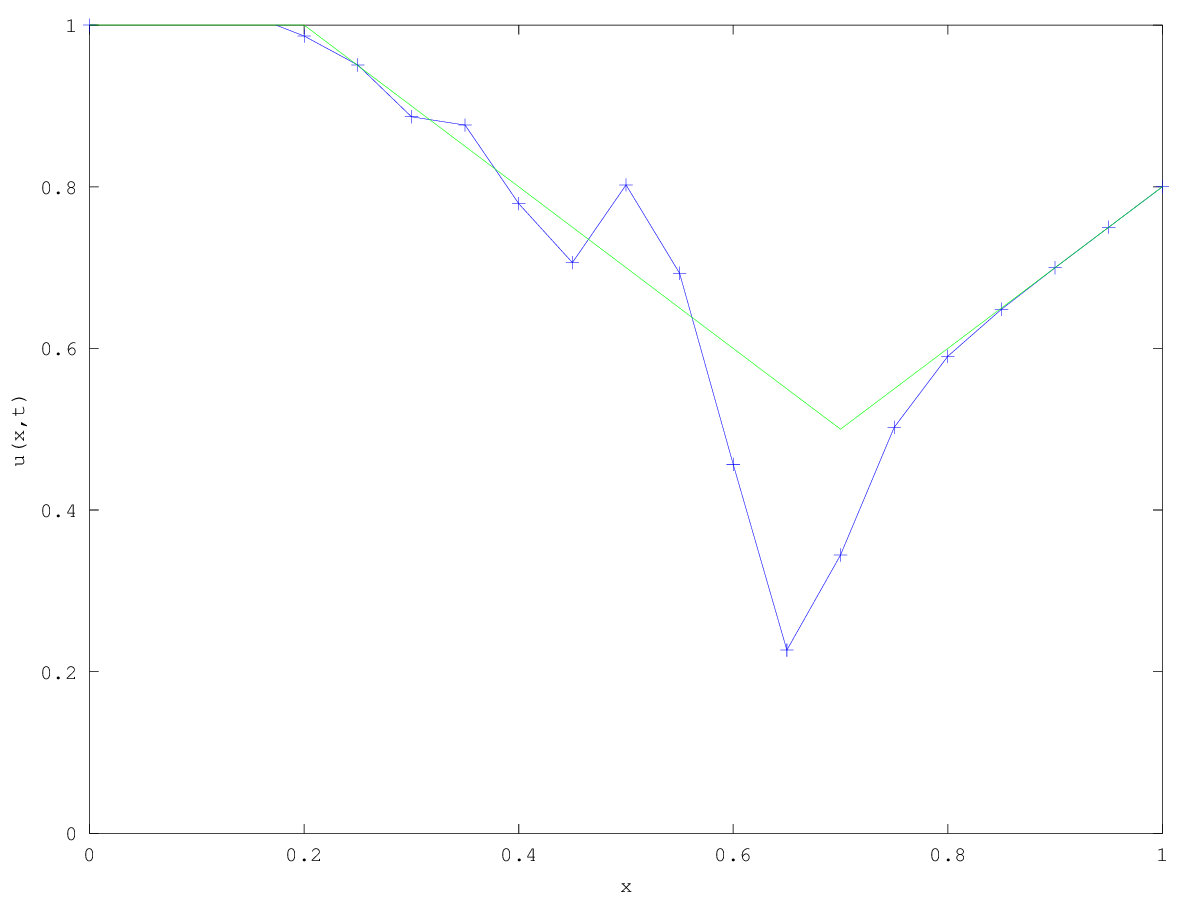
\includegraphics[width=0.95\textwidth]{diagrams/timeCoeffFTCS}
    \caption{Approximate solution to the advection equation using the undetermined time coefficient method and FTCS finite difference scheme with $\Delta t = 0.01$, $\Delta x = 0.05$, $a = 1$, $t = 0.20$.
    The solid line represents the exact solution and the line with the $\times$ symbols represents the approximate solution.}
    \label{timeCoeffWedge}
\end{figure}

\begin{figure}[p]
    \centering
    \begin{subfigure}[b]{0.95\textwidth}
        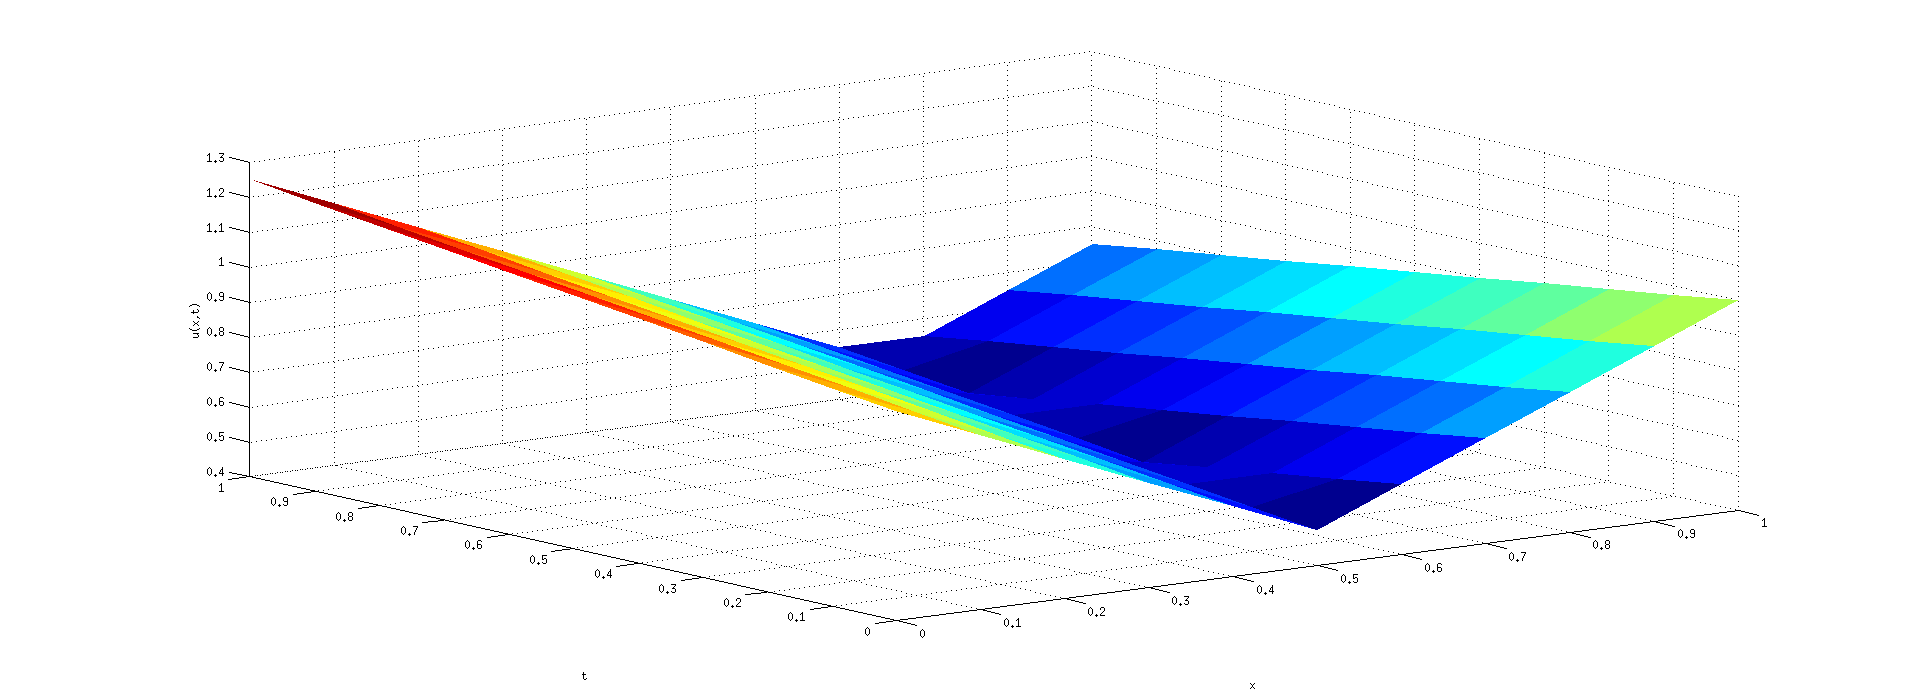
\includegraphics[width=\textwidth]{diagrams/AdvectionResultsRW}
        \caption{Approximate solution}
    \end{subfigure}
    \begin{subfigure}[b]{0.95\textwidth}
        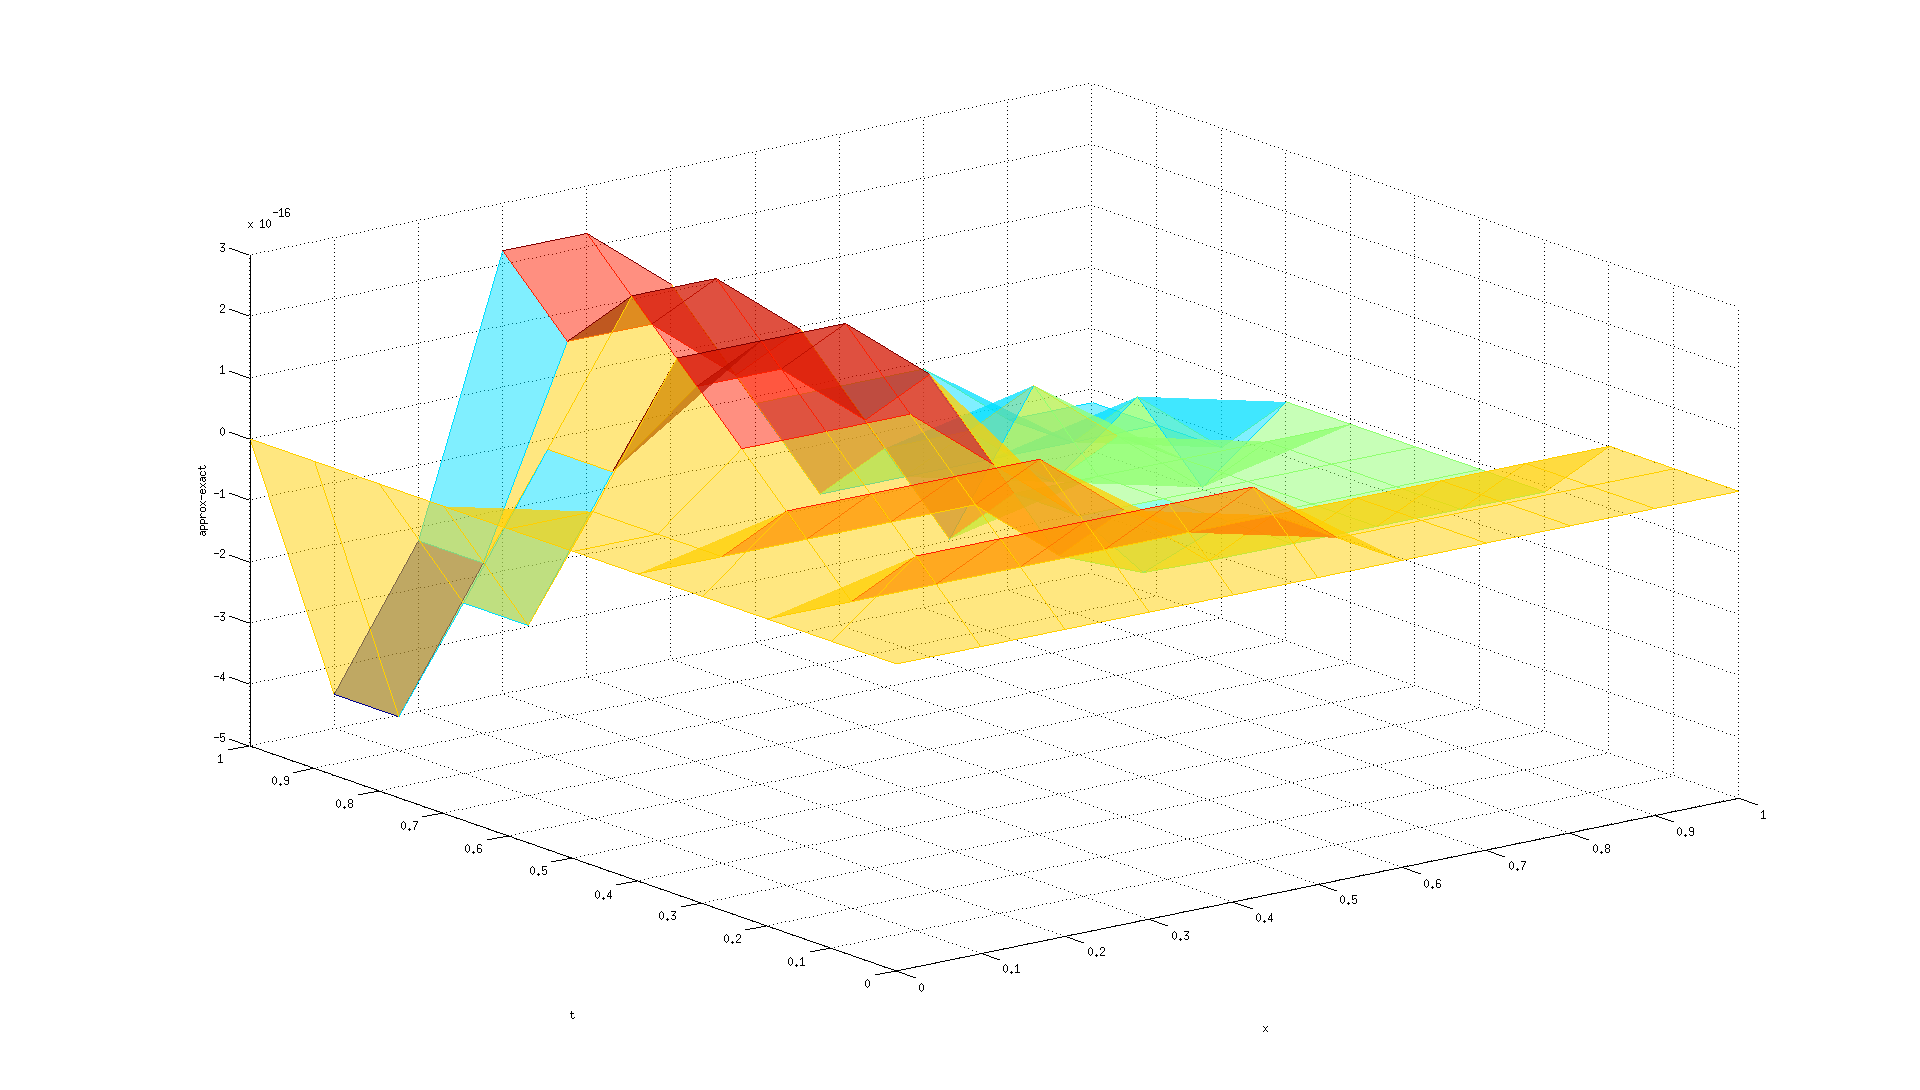
\includegraphics[width=\textwidth]{diagrams/AdvectionErrorRW}
        \caption{Errors}
    \end{subfigure}
    \caption{The results and errors computed using the Russell and Wang method applied to the FTCS finite difference scheme with wave-speed $a = 0.25$, $\Delta x = 0.1$, $\Delta t = 0.1$.}
    \label{RWFD}
\end{figure}

\subsubsection{Backwards time differencing}

The backwards time method shares the same error properties as the FTCS method ($\mathcal{O}(\Delta x^2)$ in space and $\mathcal{O}(\Delta t)$ in time) but it is unconditionally stable.

The backwards time method uses centered differences in space and backwards differences in time, making it an implicit method.

\begin{equation}
    \frac{u_i^{k+1} - u_i^k}{\Delta t} = -a \frac{u_{i+1}^{k+1} - u_{i-1}^{k+1}}{2 \Delta x}
\end{equation}

Despite its stability, the Li and Ito and unknown time coefficient methods perform equally poorly using this discretisation scheme, while the Russell and Wang method continues to perform well.
Large errors begin to appear near the interface for the Li and Ito and unknown time coefficient methods soon after beginning the simulation.
However unlike the FTCS method, these oscillations are relatively well damped through the rest of the domain most likely due to the implicit nature of this discretisation scheme.

\subsubsection{Lax-Wendroff method}

The Lax-Wendroff method is an $\mathcal{O}(\Delta x^2)$ in space and $\mathcal{O}(\Delta t^2)$ method in time method.

Its derivation involves taking a Taylor series approximation of $u(x_i,t_k +\Delta t)$ about $t$ which gives

\begin{equation}
    u(x_i,t_k + \Delta t) = u(x_i,t_k) + \Delta t \frac{\partial u}{\partial t}(x_i,t_k) + \frac{\Delta t^2}{2} \frac{\partial^2 u}{\partial t^2}(x_i,t_k) + \mathcal{O}(\Delta t^3) \label{laxWendroffTaylor}
\end{equation}

Differentiating the advection equation with respect to $t$ gives

\begin{align}
    \frac{\partial}{\partial t} \left( \frac{\partial u}{\partial t} \right) &= \frac{\partial}{\partial t}\left( -a \frac{\partial u}{\partial x} \right) \\
    \frac{\partial^2 u}{\partial t^2} &= -a \left(\frac{\partial^2 u}{\partial t \partial x}\right) \\
                                      &= -a \frac{\partial}{\partial x} \left(\frac{\partial u}{\partial t} \right) \\
                                      &= -a \frac{\partial}{\partial x} \left(-a \frac{\partial u}{\partial x}\right) \\
                                      &= a^2 \frac{\partial^2 u}{\partial x^2}
\end{align}

Substituting $\partial u / \partial t$ and $\partial^2 u / \partial t^2$ into equation \ref{laxWendroffTaylor} gives

\begin{equation}
    u(x_i,t_k+\Delta t) = u(x_i,t_k) - a \Delta t \frac{\partial u}{\partial x} + \frac{a^2 \Delta t^2}{2} \frac{\partial^2 u}{\partial x^2} + \mathcal{O}(\Delta t^3)
\end{equation}

Taking centered differences in time and truncating gives the Lax-Wendroff scheme

\begin{equation}
    u_i^{k+1} = u_i^k - \frac{a \Delta t}{2 \Delta x} \left(u_{i+1}^k - u_{i-1}^k\right) + \frac{a^2 \Delta t^2}{2 \Delta x^2} \left(u_{i+1}^k - 2 u_i^k + u_{i+1}^k \right)
\end{equation}

As with the other discretisation schemes, this is accurate away from the interface, but requires correction near the interface using one of the three correction schemes.

The Li and Ito and unknown time coefficient methods fare better with the Lax-Wendroff method, but they still cannot match the accuracy of the Russell and Wang method.
Errors in the Li and Ito and unknown time coefficient methods are more localized to point surrounding that interface than in previous methods, but there is still some clear 'rippling' on the trailing edge of the discontinuity (see figure \ref{timeCoeffLW}).
In addition, the errors at the discontinuity are much larger than the expected order in both methods.

\begin{figure}[h]
    \centering
    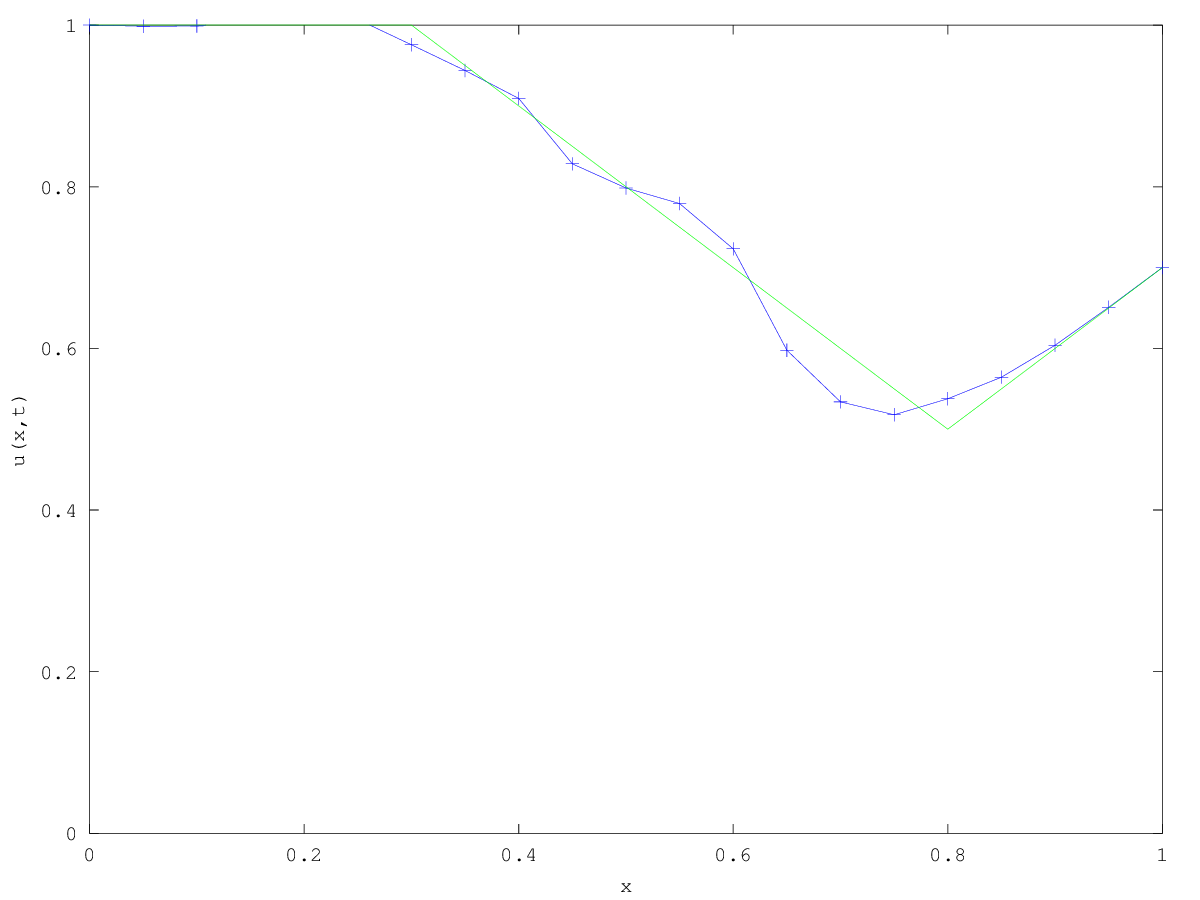
\includegraphics[width=0.95\textwidth]{diagrams/timeCoeffLW}
    \caption{Approximate solution to the advection equation using the undetermined time coefficient method and a Lax-Wendroff discretisation.
    Parameters were $\Delta t = 0.01$, $\Delta x = 0.05$, $a = 1$, $t = 0.30$.
    The solid line represents the exact solution and the line with the $\times$ symbols represents the approximate solution.}
    \label{timeCoeffLW}
\end{figure}
\subsection{The IIM for a Heaviside initial condition}

Another test problem that was used to evaluate the accuracy of these three correction methods was identical to the previous problem but with the initial condition being a Heaviside function

\begin{equation}
    u(x,0) = \begin{cases}
        1 & x < \alpha(0) \\
        0 & x \geq \alpha(0)
    \end{cases}
\end{equation}

which has exact solution

\begin{equation}
    u(x,t) = \begin{cases}
        1 & x < \alpha(t) \\
        0 & x \geq \alpha(t)
    \end{cases}
\end{equation}

This problem produced a similar pattern of errors to the previous problem.

The Li and Ito and undetermined time coefficient methods both produced fairly poor results, with large oscillatory errors evident in both the FTCS and backwards time schemes (see figure \ref{LiItoHeaviside}).
These two methods produced slightly better results using the Lax-Wendroff discretisation scheme, however there was still a large 'hump' that developed quickly on the trailing edge of the discontinuity.

As with the wedge initial condition, the Russell and Wang method proved to be accurate to the correct order with all discretisation schemes.

\begin{figure}[h]
    \centering
    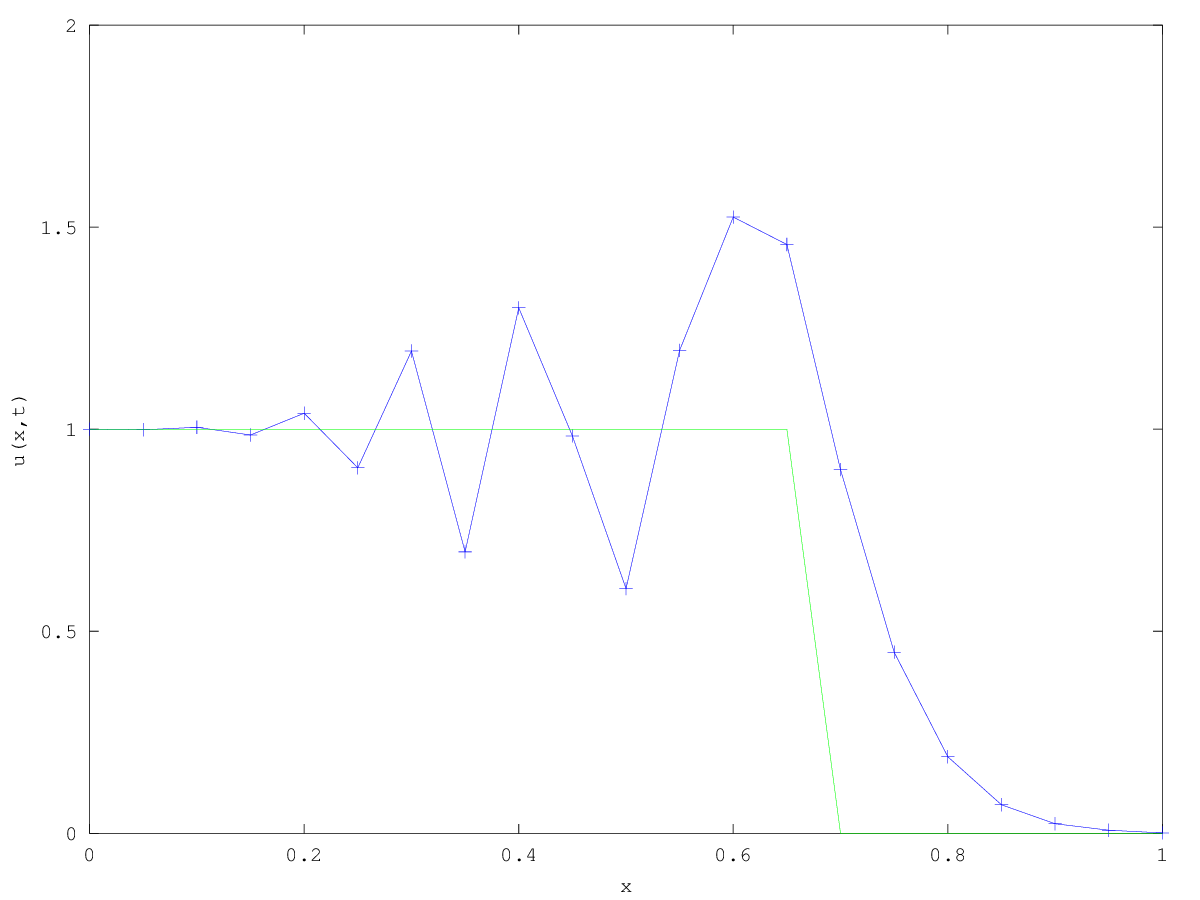
\includegraphics[width=0.95\textwidth]{diagrams/LiItoHeaviside}
    \caption{Approximate solution the advection equation using the Li and Ito method with a backwards difference discretisation.
    Parameters were $\Delta t = 0.01$, $\Delta x = 0.05$, $a = 1$, $t = 0.2$.
    The solid solution is the exact solution and the solution with the + symbols is the approximate solution.}
    \label{LiItoHeaviside}
\end{figure}
